\documentclass[12pt]{article}

%% preamble: Keep it clean; only include those you need

% if the below packages cannot be installed automatically, you can 
% download the required .sty files from CTAN and place them in the
% same location as the .tex file (or upload to overleaf in same
% location (folder) in overleaf

\usepackage{amsmath}
\usepackage{amssymb}
\usepackage[margin = 1in]{geometry}
\usepackage{graphicx}
\usepackage{booktabs}
\usepackage{natbib}

\usepackage{lineno}  % use these two lines to include line numbers
\linenumbers

\usepackage{setspace} % for doublespacing
\doublespacing


% highlighting hyper links
\usepackage[colorlinks=true, citecolor=blue]{hyperref}


\usepackage{color}
\newcommand{\blue}{\color{blue}} 
% when you make your edits in response to review/instructor comments, 
% you can indicate changes in color

%% meta data

\title{Nontrivial Transform Method in Physics-Informed Deep Learning Discovering Partial Differential Equations}
\author{Jiahua Song\\
  Department of Applied Physics and Applied Mathematics\\
  Columbia University
}

\begin{document}
\maketitle

\begin{abstract}
This paper is the summary and report of my research work on Spring 2024 in CIEN 9101. Physics-informed neural network (PINN) or Physics-informed deep learning is a new topic in machine learning. The fundamentals of PINN originated from the work of Marziar Raissi of Prof. George Karniadarkis' group in 2017 titled: Physics Informed Deep Learning:Data-driven Solutions of Nonlinear Partial Differential Equations \citep{RAISSI2019686}. It was later accepted by the Journal of Computational Physics. The complete work is separated into two main parts. One is an inverse problem; one is a forward problem. In this paper, we will introduce a new method for discovering the partial differential equations (PDE) by using the PINN method, find some interesting points raised from other related papers, and further extensions on the papers we are interested in for finding new PDEs based on the dataset, and do some code realizations for my new method as much as I can.  

\noindent\textbf{Keywords}: Physics-informed neural network (PINN), PDE, data-driven, inverse problem.
\end{abstract}


\section{PINN Discovering PDEs}
\label{sec:intro}
The proper definitions of forward and inverse problems can be explained as follows: a forward problem, where the cause is known, and the outcome state or observation is obtained based on existing models and laws, and an inverse problem, where the outcome state or observation is known to invert the cause. Examples of forward problems include that you give someone a cake, and based on modeling, you know that he has the facial expression and reaction after he tastes your cake; the inverse problem is that a person has a kind of facial expression and some reactions. One can ask him what happened, and we might surmise that maybe he tasted a delicious cake. But maybe it wasn't, maybe the guy got enlightened by some coincidence to finish his work or get some other good surprises. This phenomenon is what is known as the ill-posedness of the inverse problem. Other examples of forward problems include designing the program parameters of an airplane, which can then be simulated so that the performance of the airplane can be known, and the inverse problem, which is the inverse of what design solution should be given based on the design requirements of the airplane. Therefore, the engineering community usually refers to the forward problem as the simulation problem and the inverse problem as the design problem. For a PDE equation, we define a forward problem as knowing the PDE equation and solving the PDE equation in the field and an inverse problem as knowing some observations in the field and inverting the values of the coefficients/parameters of the optimal PDE equation. However, this is a very narrow and basic definition, and we will extend it later. From a certain point of view, the forward and inverse problems are symbiotic problems of a set of systems, which can also be regarded as the opposing poles or as the cycle of the chicken laying an egg and the egg laying a chicken. In short, the two are opposites but united and mutually reinforcing.

\subsection{Forward Problem}
As I said earlier, for the PDE problem, the forward problem of PINN is to solve the solution in the field based on the existing PDE. How to do it? Simply build a neural network to learn the properties of the PDE. Specifically, it is to establish a mapping between the time coordinate $t$ and the spatial coordinates $x$ and $y$ solutions, i.e., $G: x\to y$. Of course, the stationary process has no $t$.

It is well known that the training of neural networks requires an objective function, so how does this process give the objective function? It's simple: the PDE equation is actually a loss function; if it does not satisfy the equation relationship, it will produce loss, so put your neural network's $t,x$ and $\hat{y}=G(x,y)$ into the PDE to obtain the loss. Here, one may wonder how this is different from traditional machine learning.

The difference lies in a very interesting design: the PDE has (higher-order) derivative terms, and we don't know their values yet. In fact, we can't construct a PDE loss function, so how do we know the values of these derivatives? This relies on another property of neural networks, which is being completely differentiable. Just do the backward gradient propagation, calculate the gradient term of the neural network, and put it into the PDE loss. By training in this way, the resulting model $G$ can fully satisfy the mathematical laws reflected in the PDE. A simple example of the process is shown in figure \ref{fig:FP}, where $\sigma$ is the activation functions used to get the form a $u(t,x)$ and $v(t,x)$, and differential operators are treated as neurons to get the PDE or loss functions. 

\begin{figure}[!t]
  \centering
  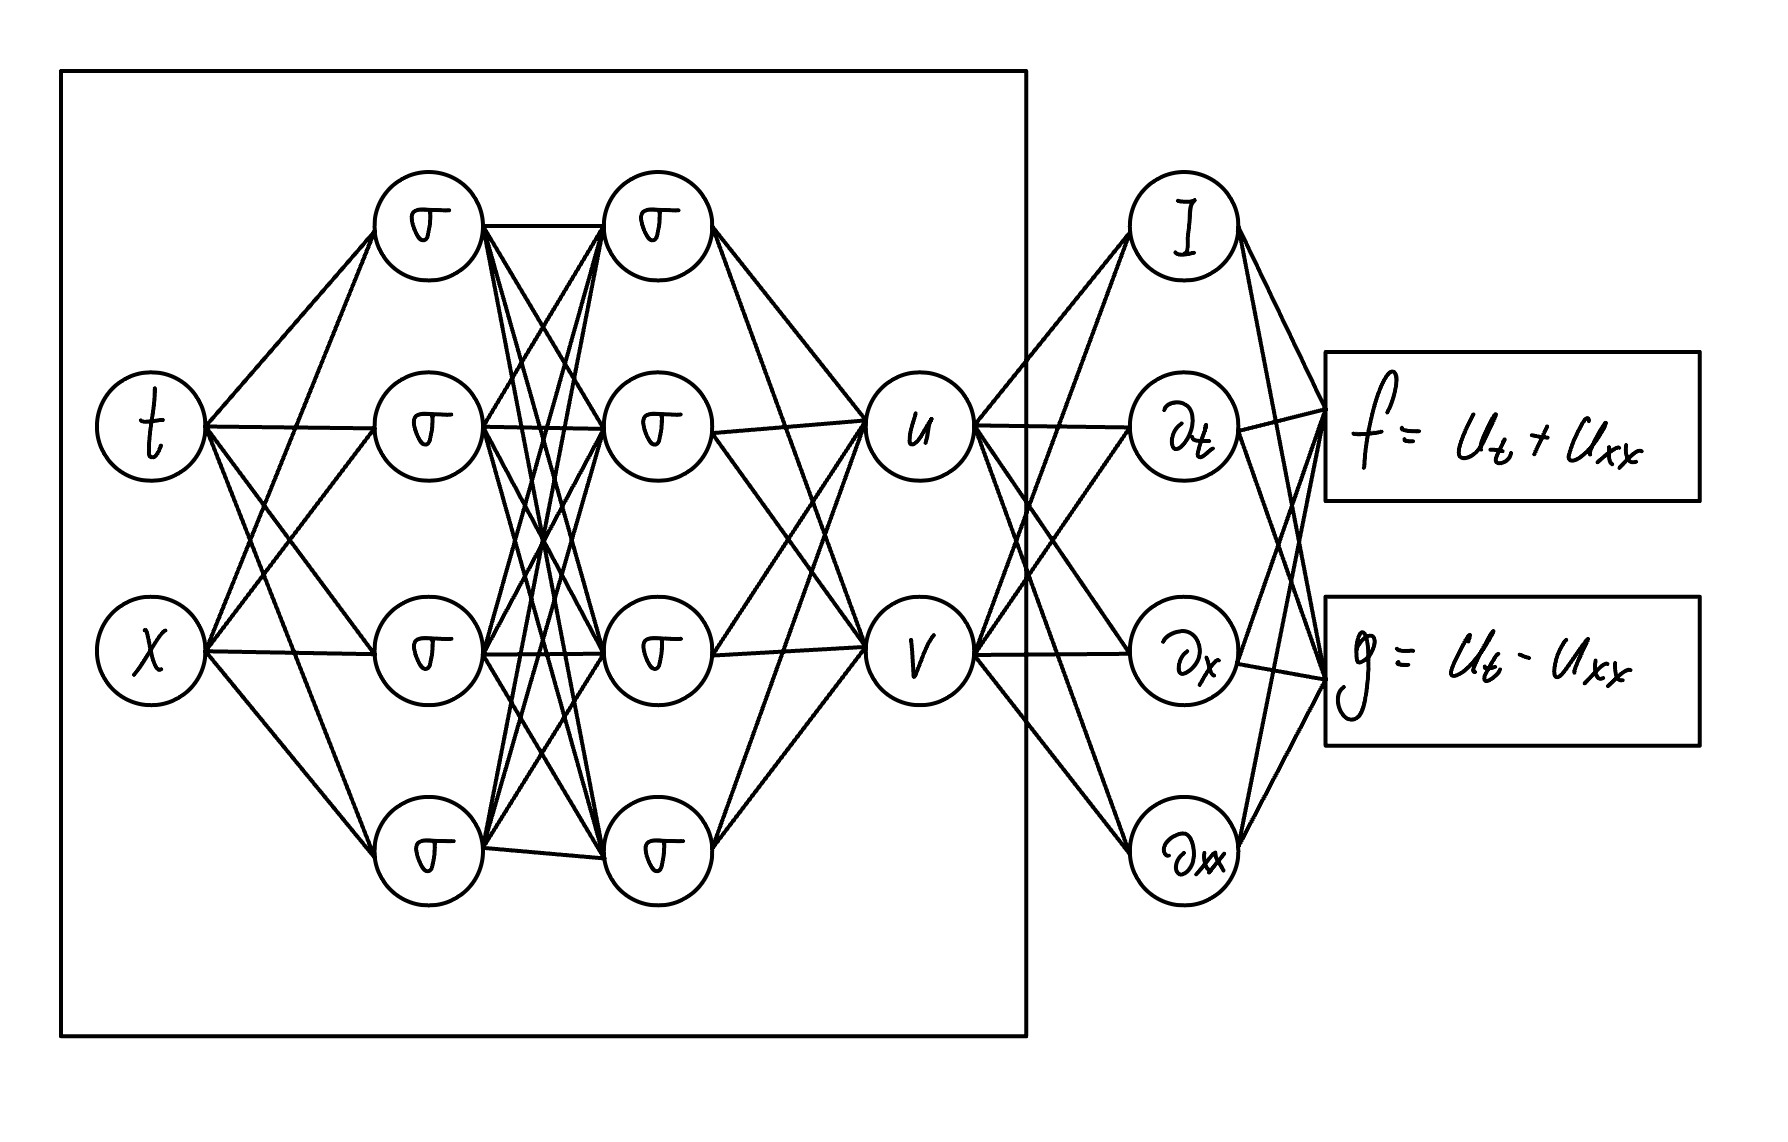
\includegraphics[width=\textwidth]{FP.jpeg}
  \caption{Neural network of a Forward Problem in PINN.}
  \label{fig:FP}
\end{figure}

From a mathematical point of view, the biggest difference between it and traditional machine learning is that on top of requiring the $0$-th order constant term to be consistent with the system; it also requires the higher order gradient term to be consistent with the system. From the perspective of Taylor expansion, it clearly has higher accuracy because it better satisfies the high-dimensional characteristics of the system. From the perspective of machine learning and problem adaptation, the use of neural networks rather than other machine learning methods is also a very insightful design, as the microscopic nature of neural networks brings about the feasibility of gradient solving, while the ease of engineering implementation is brought about by the autograd of existing frameworks such as PyTorch, which effectively avoids the complexity of methods using, for example, a Gaussian process or a decision tree. From a purely machine learning point of view, PINN is a variant of reinforcement learning; the so-called PDE system is nothing more than a kind of environment to provide evaluation. PINN, this PDE solver, in fact, is a policy model. For similar work, you can refer to Google's optnet, which is also a work of $2017$. It is because the PDE equations already contain all the information (a one-world model) that, when solving a forward problem, PINN requires no data at all, just random sampling in space and time steps, and then letting the PDE equations evaluate whether the neural network's modeling is accurate or not; or the real data is an intermediate quantity based on the PDE's loss function. In light of this, it has been claimed that PINN is a type of meshless method. This is inevitable, as it learns the properties of the entire PDE system rather than a simple coordinate mapping.


\subsection{Inverse Problem}
The task of the PINN in solving the inverse problem is to invert the hyperparameters (coefficients) of the terms in the PDE. The setting of this problem means that we do not have real and reliable PDE equations to make a judgment . Therefore, actual observations (values of the field) are needed to provide the loss function. In short, we are picking the best of a family of PDEs to fit the actual system (based on the laws reflected in the actual observations). In order to do this, we need to add these coefficients to the learnable parameters as well so that PINN acts as a player (fitting the PDE system properties) and a referee (finding the best-fitting PDE coefficients to fit).

From a certain point of view, the PINN solving the inverse problem in the original article is not actually a complete solution of the inverse problem because the forward problem is to learn the whole solver, so the corresponding inverse problem should be to learn the whole PDE, not just to compute the coefficients. This is actually a historical limitation because if we want to learn the whole PDE, the operation operators such as addition, subtraction, multiplication, division, and higher-order differentials are not differentiable and cannot be embedded into neural networks. The authors realized at the time that they could not embed these things in a neural network framework. Based on the author's realization of this, his approach takes a back seat. To learn these things, we need to introduce another thing called symbolic learning. Over the years, there have been some interesting things that have broken the previous search explosion logjam, and some interesting things have been done by Dr. Miles Cranmer of Princeton and the previous alphatensor of DeepMind. 


Recently, we found some new methods to combine deep learning with symbolic regression, enabling the possible ways to discover the parametric PDEs from data \citep{Zhang2022DeepLA}. \citet{Zhang2022DeepLA} proposed a method called Parametric Equation Learner (PEQL) to perform neural network-based symbolic regression to parametric equations. The PEQL method is proven to be useful in analyzing systems that we know are partially governed by an analytic equation and partially governed by some other mechanism that may be complex. \citet{PhysRevResearch.4.023174} proposed a Symbolic genetic algorithm (SGA-PDE) method to discover the open-form PDEs directly from data. The framework is that given data and candidates of PDE symbols, we can do a genetic algorithm for binary trees. After crossover, mutation, and replacement, we can get the optimal (measured by the sparse regression) PDE expression governing the given data. The method is successfully tested by finding nonlinear Burger's equation, Korteweg–de Vries equation, and the Chafee-Infante equation \citep{PhysRevResearch.4.023174}. \citet{richterpowell2022neural} proposed a new model called Neural Conservation Laws (NCL) that integrate divergence-free conditions in the neural architecture, ensuring that the continuity equation is always satisfied, thus enabling precise simulation and analysis of fluid dynamics and other related fields. In the industry, the method beats the CFD in the computational sense by avoiding penalty terms. It also enhances the accuracy and reliability of the model in scientific simulations \citep{richterpowell2022neural}.

These developments provide many interesting perspectives on understanding and solving Raissi's problem. The results guarantee the accuracy and efficiency of discovering PDEs from data, allowing researchers to deal with complicated problems in academia and industry. 



\section{Interesting points in Related Papers}
\label{sec:interets}

In the original work of discovering PDEs. \citet{RAISSI2019686} considered the parametrized and nonlinear PDE form
\begin{equation}
    \label{eq:GF}
    u_t + \mathcal{N}[u;\lambda]=0, \quad x\in \Omega, t\in [0,T]
\end{equation}
where $u(t,x)$ denotes the solution, $\mathcal{N}[\cdot;\lambda]$ is a nonlinear operator parameterized by $\lambda$, and $\Omega$ is a subset of $\mathbb{R}^D$. 

\citet{RAISSI2019686} separates it into a continuous time model and discrete-time model to optimize the parameter $\lambda$ for the nonlinear operator based on the network built by $f=u_t + \mathcal{N}[u;\lambda]$. This is introduced in \ref{sec:intro} that the method is limited to be a traditional neural network problem. It can be further extended into varying not only parameters but also the parametric equations \citep{Zhang2022DeepLA}. Even more generally, the operators use the symbolic learning method \citep{PhysRevResearch.4.023174}. 





\section{Extension on new PINN Method}
\label{sec:meth}

In addition to the symbolic learning mentioned above, the use of PINN needs to pay attention to some other issues; for example, we know that the solution of a PDE equation depends on the boundary conditions and initial conditions. However, the learning process of PINN does not mention these because, given a system, the boundary and initial conditions are fixed, and these things are taken as a priori and not put into PINN. Therefore, what PINN learns in its study is the operating characteristics of a given PDE for a given boundary and initial conditions. Some people often yell that PINN does not have a generalization, but in fact, we do not let it learn generalization. Then, how to make the method with generalization capable well may depend on the boundary conditions and initial conditions. It is worth spending time researching how to add the conditions. 

Another means is to use neural operators; the very first neural operator method, Deeponet, was also popularized by Karniadarkis. The most initial theoretical construction was proposed by \citet{392253}. More advanced algorithms came later, namely the Fourier Neural Operator and its derivatives. In a nutshell, the network structure of these operator methods ensures that the learning process is consistent with Green's formula for solving PDEs and, therefore, can satisfy all the properties of PDEs, but in fact, their learning process, I think, is sort of incorporating boundary conditions.

The challenge of solving the inverse problem also raises interesting questions. For instance, different boundary conditions could lead to varying optimal coefficients (members of the PDE family). Even for the same system, there could be an optimal case at different times. This variability in the inverse problem presents a promising avenue for future research, one that could significantly contribute to our understanding of PINN's generalization capabilities. 

Here, I extend the PINN and symbolic regression techniques to a new method. In principle, the symbolic learning method mentioned in the paper of \citet{PhysRevResearch.4.023174} uses the idea of a genetic algorithm. It starts from a set of random initializations of PDEs and fits the data with minimum residual. Then, we compute the adaptability (measured by quantities of interest) of the current living individuals, and based on the adaptability, we give them a probability to pass their PDE expression to the next round. Based on the probability distribution, we can randomly cross over the expressions to form a new PDE expression that also relates to the original data and randomly mutate the PDE expression. We use the new generation of PDEs to do the same process as above. Finally, we set a threshold like error less than $\epsilon = 10^{100}$ with respect to a norm of interest like Frobenius norm for exiting the iteration.

The idea of mimicking the genetic expression is heuristic. However, it doesn't solve the ill-posedness problem, which is caused by the nature of the inverse problem. I propose a new method called ${\bf{Nontrivial\text{ }Transformation\text{ }  Method}}$ to extend the ability to find more potential PDE expressions governing the given data. 

The idea of the Nontrivial Transformation Method also comes from nature as well. The limitation of using the genetic algorithm is that one can mutate and crossover to find new PDE expressions and optimize it to get the least residual one expression. However, one cannot simultaneously say that there is a set of relations that connect these optimal expressions when it actually is. The hidden relation reasonably comes from the fact that no universal optimal expression governs a dataset forever and with respect to different references. It is similar to having a different perspective on the same physical phenomena, like light, which can be viewed as partials and waves. Thus, we just need to find the nontrivial transform such that under that system, we can find the relation of the optimized PDE expression by symbolic regression; thus, we can get potentially new PDE expressions based on the relation. 

Intuitively, the genetic algorithm can be viewed as a current-time optimal solution. If you do symbolic regression at different times, we will get different governing PDE equations, and if we change the coordinate system, like from finite to infinite dimensions or some weird topological space, the expression may be different as well. However, they all come from the same real-world data with the same parameterized description. It is reasonable that there might be some connections to the discrete set of optimal PDE equations, and the equations between two discrete objects can be described by a new PDE expression, which may not been discerned by the random sampling of the genetic algorithm. Based on this intuition, instead of doing symbolic regression point-wisely, we do it in a uniform way. The simplest illustration is the Van Der Pol Oscillator.
\[
\frac{d^2x}{dt^2}+\mu (1-x^2)\frac{dx}{dt}+x=0
\]
Same as 
\[
\begin{bmatrix}
    \Dot{x}\\
    \Dot{y}
\end{bmatrix}=\begin{bmatrix}
    y\\
    \mu(1-x^2)y-x
\end{bmatrix}
\]
It is not so obvious if we use a Cartesian coordinate to express the potential limit cycle, but if we transform it into a polar coordinate, it is very obvious. 
\[
\Dot{r}=\mu (1-r^2 \sin{\theta})r \cos{\theta}=0
\]
However, what we want to solve is not the function $x(t),y(t)$. We will treat $x(t),y(t)$ as the PDE expressions, and the oscillatory relation is the hidden relation of the PDEs in the data. We also use the PEQL to incorporate the PDE set with hidden relations. PEQL method comes from the work of \citet{Zhang2022DeepLA}. Theoretically, the SGA-PDE will give the correct discrete PDE expressions of PEQL after NTM. SGA-PDE comes from the work of \citet{PhysRevResearch.4.023174}. The whole framework of this method is shown in Figure \ref{fig:NTM}. If there is a discrepancy between these two outcomes, there must be some new relations or variables we do not include as long as the transform in NTM is well-defined and satisfies the properties needed in the given circumstance. This discrepancy can be further studied, but for now, we can use the discrepancy as a loss function to form a neural network and get the optimal PDE expression set if the discrepancy exists. 

\begin{figure}[!t]
  \centering
  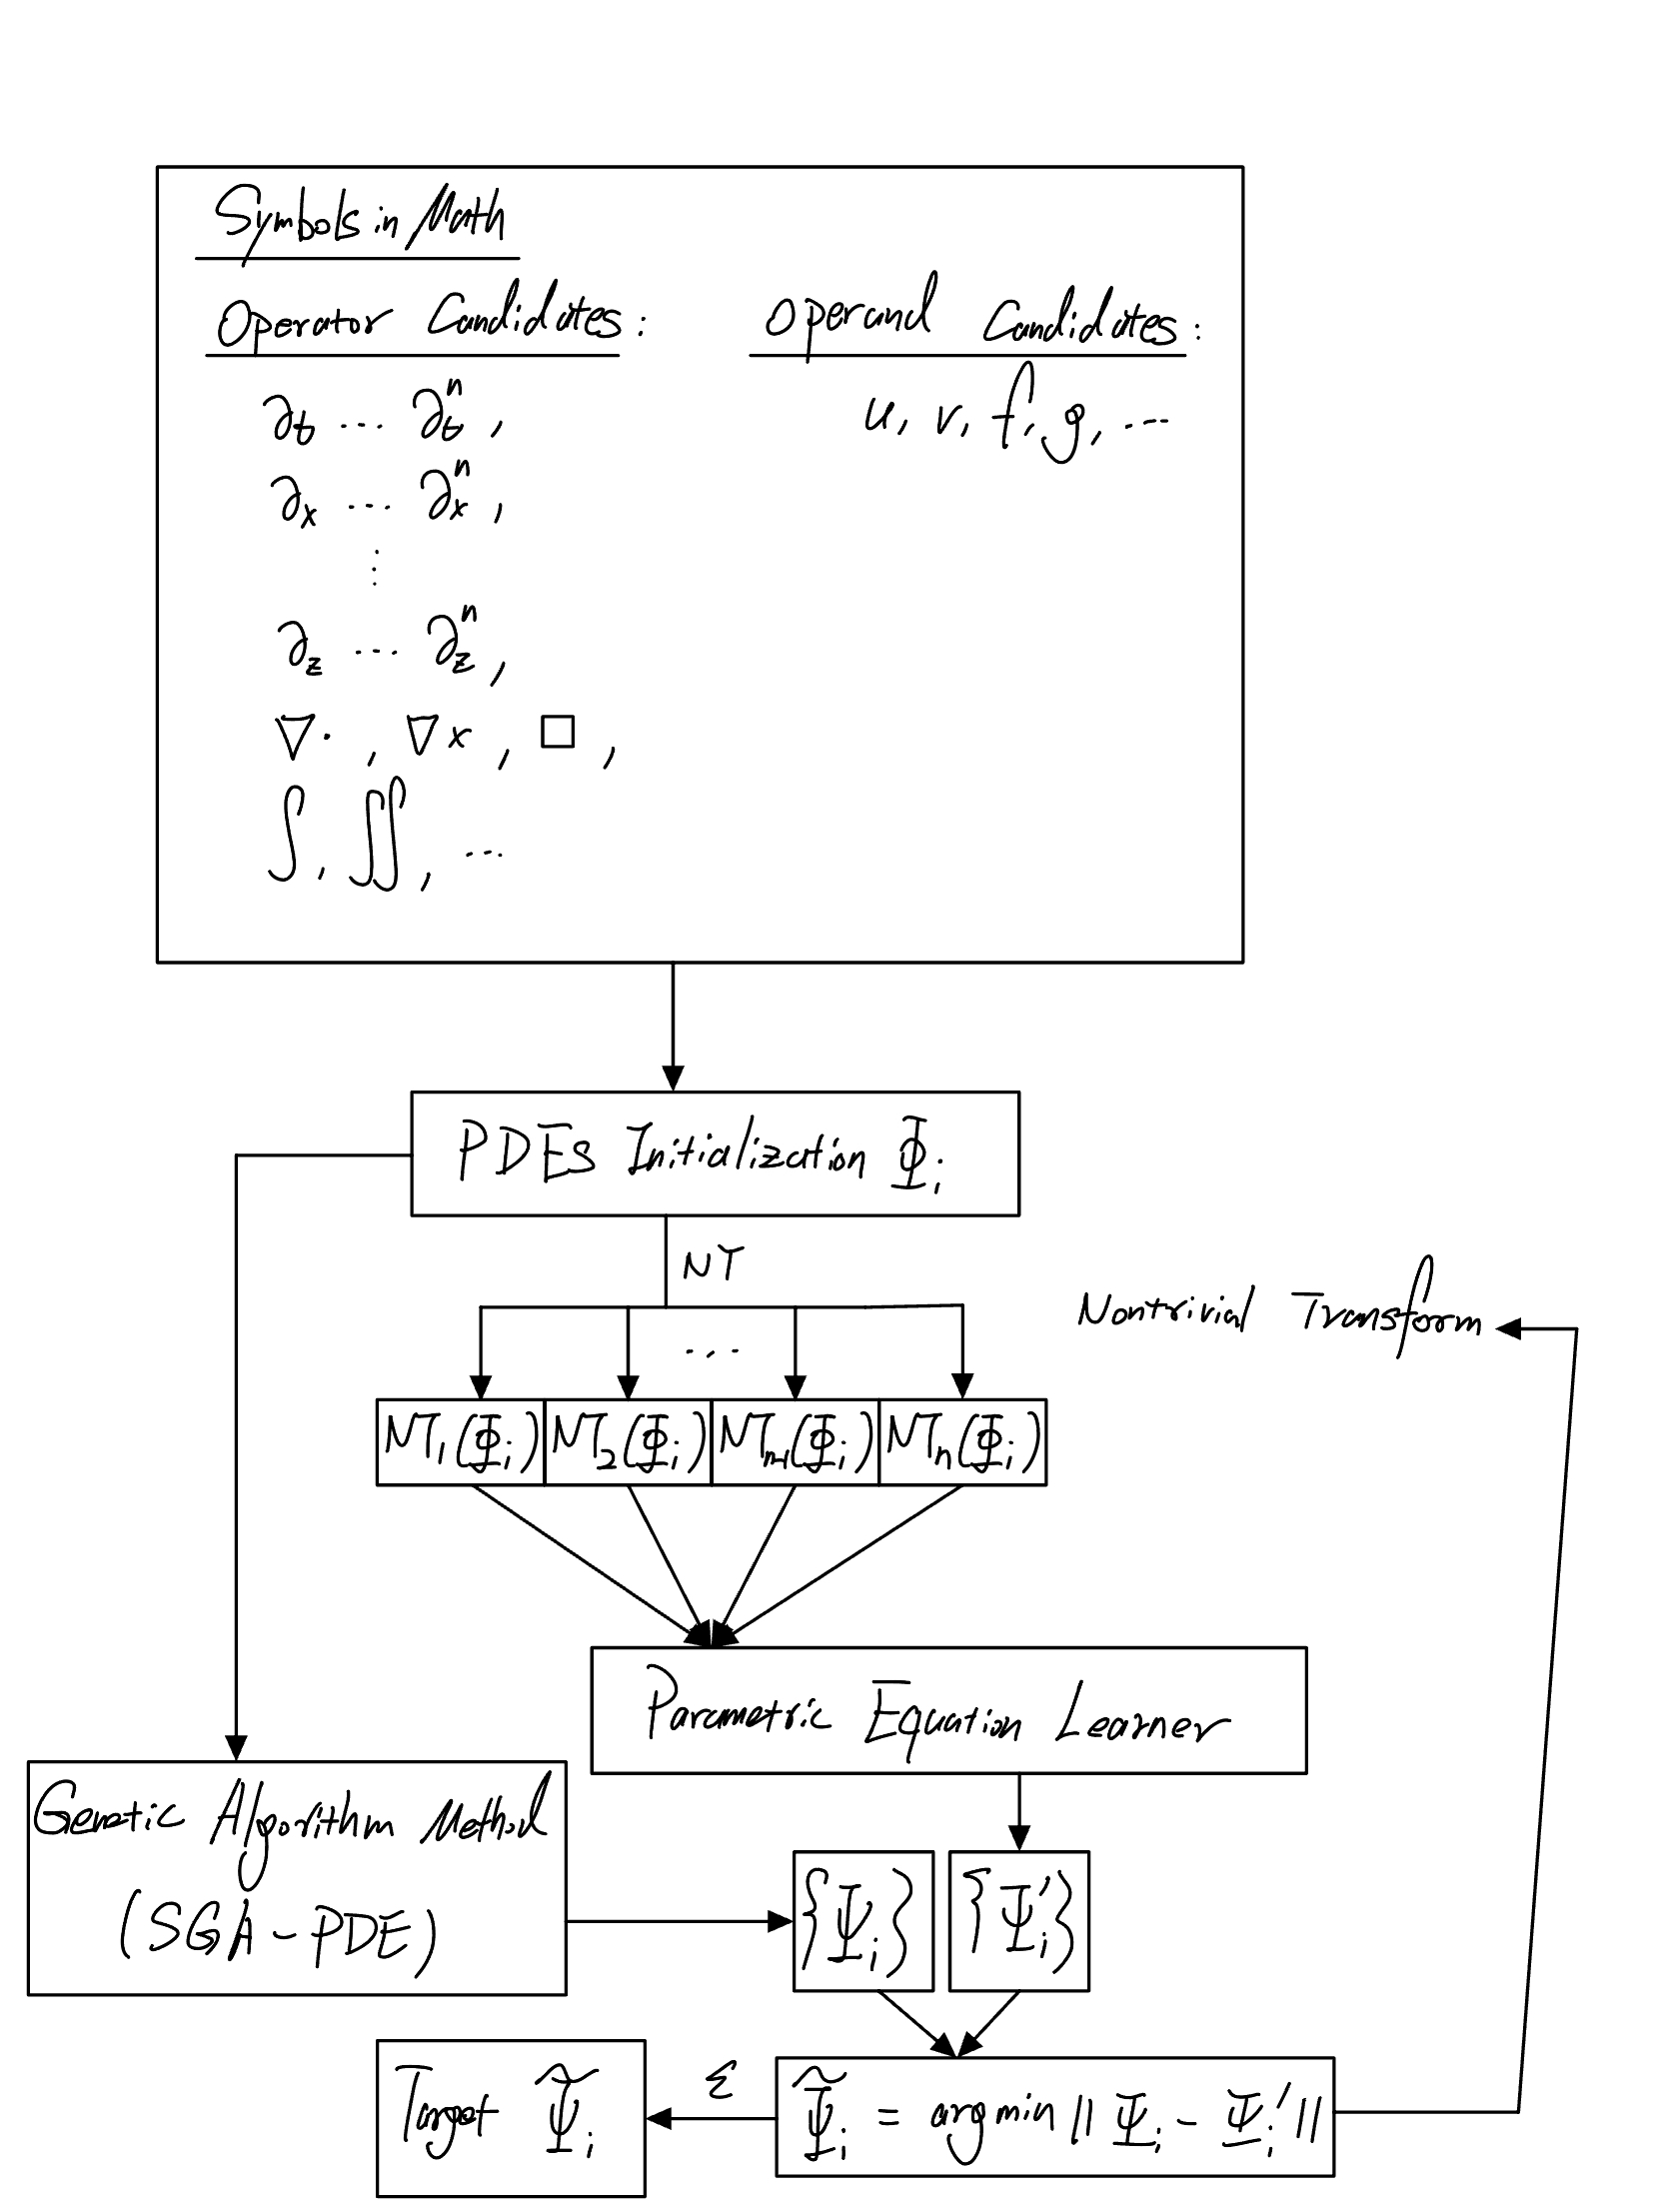
\includegraphics[width=\textwidth]{NTM.jpeg}
  \caption{Nontrivial Transformation Method Framework.}
  \label{fig:NTM}
\end{figure}




\section{Realization Results}
\label{sec:resu}
Given random sampling data points on PDE $u_t=u_{xx}$, we proceed with the SGA-PDE to get discrete PDE expression $0.65u_t+0.35u_{xx}=0$. It is not quite correct since the nature of genetic programming mutates and crossover the expression no matter whether one is optimal or not. Based on PEQL, we see that the result is pretty accurate with residual evaluated $0.0011529753683134913$. Finally, I tested the NTM also for $u_t=u_{xx}$, and the result and conclusion are promising, as shown in the code part in GitHub. 

\section{Discussion}
\label{sec:disc}
The paper focuses on the theory of NTM, which is reasonable in theory. However, there are some problems in the coding part since I just used the simplest example to illustrate the method. The result may not be robust and valid in certain circumstances. It is worth some time to do further research on the coding realization of other PDE discoveries using NTM. 


\bibliography{refs}
\bibliographystyle{mcap}

%\section*{Appendix} %optional

\end{document}